
%(BEGIN_QUESTION)
% Copyright 2011, Tony R. Kuphaldt, released under the Creative Commons Attribution License (v 1.0)
% This means you may do almost anything with this work of mine, so long as you give me proper credit

This diagram shows a sample system for a set of CEMS analyzers:

$$\includegraphics[width=15.5cm]{i03420x01.eps}$$

Identify and explain the consequence of a technician accidently leaving hand valve \#7 (V7) shut.  Assume everything else in this analyzer system is operating as it should.

\vskip 50pt

Identify and explain the consequence of the sample line heat tracing failing (turning off), being as specific as you can.  Assume everything else in this analyzer system is operating as it should.  

\vskip 50pt

\underbar{file i03420}
%(END_QUESTION)





%(BEGIN_ANSWER)

Identify and explain the consequence of a technician accidently leaving hand valve \#7 (V7) shut.  Assume everything else in this analyzer system is operating as it should.  {\bf The chemiluminescence detector will output a 0 ppm measurement for NO$_{x}$ because it cannot produce any ozone to react with NO$_{x}$ gases in the sample.}

\vskip 10pt

Identify and explain the consequence of the sample line heat tracing failing (turning off), being as specific as you can.  Assume everything else in this analyzer system is operating as it should.  {\bf Condensate in the sample line may freeze during cold weather, plugging the line and causing all CEMS analyzers to receive stale (old) sample gas.}

\vskip 10pt

I recommend granting half-credit for each correct explanation (5 points each).

%(END_ANSWER)





%(BEGIN_NOTES)

{\bf This question is intended for exams only and not worksheets!}.

%(END_NOTES)

